\documentclass[../main.tex]{subfiles}

\begin{document}
\section{Programmazione Reattiva}
Con programmazione reattiva si intende un paradigma di programmazione dichiarativo basato sullo stream dei dati e sulla propagazione dei cambiamenti, fortemente correlato con i pattern Observer, Reactor ed il paradigma Event-Driven.
Un programma reattivo è costruito definendo la logica della computazione ma non il flusso di controllo, il quale è definito dal verificarsi degli eventi.

\subsection{Modelli di valutazione}
Il cambiamento di un valore deve essere propagato automaticamente a tutte le sue dipendenze, azionando la ricomputazione attraverso la notifica. I modi possibili per la propagazione dei cambiamenti e quindi la loro valutazione sono:
\begin{description}
    \item[Push:] (paradigma consumer) I consumatori ricevono dalle sorgenti i dati non appena questi diventano disponibili. 
    \item[Pull:] (paradigma producer) I consumatori richiedono regolarmente i dati ai produttori.
    \item[Push-Pull:] I consumatori ricevono una notifica che descrive il cambiamento e per ottenere le informazioni necessarie devono richiederli ai produttori.
\end{description}
Il modello Push-Pull, chiamato anche backpressure, consiste in una modifica del modello Push che permette ai consumatori di inviare segnali di feedback ai produttori riguardanti l'andamento della propagazione del cambiamento. Il produttore può richiedere (Pull) quanti elementi desidera se questi sono disponibili, ma se questi non sono disponibili vengono ricevuti (Push) non appena lo diventano.

\subsection{Observable e Stream}
Con observer si intende l'entità che si sottoscrive ad un observable in modo da essere notificato e reagire ad ogni elemento che esso emette. Mentre gli observable rappresentano quindi degli stream di dati asincroni che possono essere concatenati insieme (dipendenze) per definire in modo dichiarativo nuovi stream più complessi.

\begin{figure}[H]
\centering
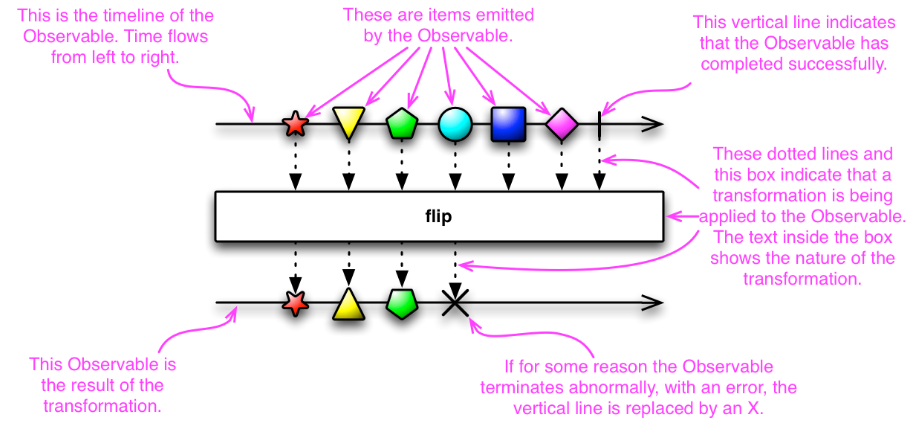
\includegraphics[width=1\textwidth]{img/observable1.png}
\caption{Esempio di Observable - Marble Diagram}
\end{figure}

Le tipologie di stream sono classificate in base a quando l'observable inizia ad emettere i dati:
\begin{description}
    \item[Hot:] L'observable inizia ad emettere dati appena viene creato (modalità eager) e continua senza considerare quanti observer sono registrati. Quando un observer si registra riceve dati solo dal quel momento in poi a meno che non si faccia uso di altri meccanismi come cache/replay.
    \item[Cold:] L'observable inizia ad emettere dati solamente quando si registra almeno un observer (modalità lazy). Ogni volta che un nuovo observer si registra l'observable riiniza ad emettere i dati da capo garantendo gli stessi dati a tutti gli observer.
    \item[Connectable:] L'observable accetta sottoscrizioni dagli observer ma inizia ad emettere dati solamente quando viene invocato l'apposito metodo.
\end{description}

\section{FP + RP = FRP}
Il multiparadigma chiamato Functional Reactive Programming (FRP) consiste nella combinazione dei paradigmi funzionale (FP) e reattivo (RP): permette infatti di manipolare stream di dati in modo asincrono con backpressure non-bloccante utilizzando le feature del paradigma funzionale come immutabilità, assenza di side-effects, referential transparency, ...).

\subsection{Caratteristiche paradigma FRP}
I concetti chiave alla base del paradigma FRP sono i due tipi di dato \textit{Behavior} e \textit{Event}, e tipicamente dieci operazioni basiche chiamate \textit{primitive}. Alcuni sistemi FRP non fanno distinzione, modellando entrambi i due tipi di dato con il concetto \textit{Signal}:
\begin{description}
    \item[Behavior] - Modella valori che variano nel tempo. Altri sinonimi di behavior sono \textit{Property} o \textit{Cell}. I behavior modellano lo stato, valori che possono essere ottenuti in qualsiasi momento.
    \item[Event] - Modella un sequenza di eventi in ordine cronologico. Altri sinonimi di event sono \textit{Stream} o \textit{Observable}. Un evento viene propagato attraverso uno stream in un preciso momento, in questo caso si dice che lo stream è attivo (\textit{fired}). Gli stream a differenza dei behavior modellano i cambiamenti dello stato, valori che possono essere ottenuti solamente nell'istante in cui uno stream è attivo.
\end{description}

Le seguenti dieci primitive sono le operazioni basiche che tipicamente sono presenti in un sistema FRP:
\begin{description}
    \item[Map] - Primitiva che genera un nuovo stream applicando una certa funzione ad ogni evento emesso all'attivazione di uno specifico stream.
    \item[Merge] - Definisce uno stream unendo gli eventi di due stream. Questa primitiva è chiamata anche \textit{union} o \textit{append}.
    \item[Hold] - Converte uno stream in un behavior inserendo nel behavior l'ultimo evento ricevuto dallo stream. Questa primitiva è chiamata anche \textit{toProperty}.
    \item[Snapshot] - Cattura/Combina il valore di un behavior nell'istante in cui si attiva uno specifico stream. Questa primitiva è chiamata anche \textit{withLatest} o \textit{attach}.
    \item[Filter] - Definisce uno stream con una certa logica di attivazione tramite la definizione di un predicato. L'evento viene propagato solamente se è soddisfatto il predicato.
    \item[Lift] - Primitiva simile alla primitiva \textit{map} ma che opera sul singolo behavior. Definisce un operazione da un valore contenuto in un behavior verso un altro tipo di "container" come ad esempio \textit{List} o \textit{Optional}.
    \item[Never] - Definisce uno stream che non si attiva mai.
    \item[Constant] - Un behavior definito tramite questa primitiva assume un valore costante che non può essere cambiato.
    \item[Sample] - Estrae il valore di un behaviour.
    \item[Switch] - Primitiva, chiamata anche \textit{flatten} o \textit{join}, che permette di modificare dinamicamente il grafo delle dipendenze.
\end{description}

\subsection{Lifecycle Programma FRP}
Un programma FRP è quindi un insieme di behavior e event, costruito partendo da valori statici (che non variano nel tempo) e/o altri behavior/event. Questi sostituiscono il \textit{pattern Observer} fornendo un sistema per programmare logica event-driven in modo componibile/modulare, ovvero definire reazioni al verificarsi di un evento (un input o stream di dati). L' esecuzione di un programma FRP può essere suddivisa in 3 step:
\begin{description}
    \item[Inizializzazione] - Allo startup del programma gli statement vengono convertiti in un grafo orientato in-memory in modo da rappresentare le dipendenze tra gli stream di dati.
    \item[Esecuzione] - Per il resto del tempo d'esecuzione il programma attende un input/cambiamento e produce un output valutando le dipendenze del grafo.
    \item[Modifica Grafo] - Nulla vieta di modificare dinamicamente le dipendenze tra gli stream di dati e quindi il grafo orientato che le rappresenta.
\end{description}

\begin{figure}[H]
\centering
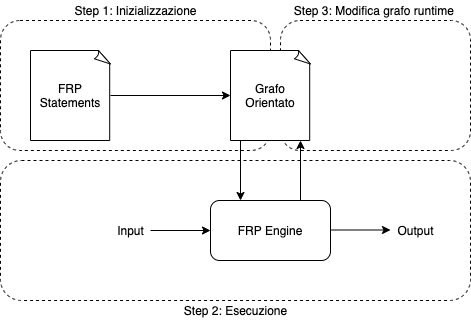
\includegraphics[width=0.8\textwidth]{img/frp-scala1.png}
\caption{Lifecycle Programma FRP}
\end{figure}

\subsection{FRP vs RP}
In RP "\textit{everything is a stream}" mentre in FP "\textit{everything is a function}". Come indicato nella documentazione della libreria ReactiveX riferendosi al paradigma reattivo: "\textit{It is sometimes called functional reactive programming but this is a misnomer. ReactiveX may be functional, and it may be reactive, but “functional reactive programming” is a different animal. One main point of difference is that functional reactive programming operates on values that change continuously over time, while ReactiveX operates on discrete values that are emitted over time.}".

Lo stesso discorso vale per i \textit{Reactive Streams} i quali condividono alcuni aspetti col paradigma FRP ma sono una "cosa" diversa. Per definizione infatti "\textit{Reactive Streams is an initiative to provide a standard for asynchronous stream processing with non-blocking back pressure}" ma sono basati sullo stesso concetto del paradigma RP, ovvero valori/eventi che si verificano in un certo momento discreto.

% fare esempio mouse: in rp il mouse è un observable che emette eventi al cambio della posizione e al quale è possibile sottoscrivere una azione, in frp il mouse è rappresentato tramite due variabili che cambiano valore nel tempo, x e y sono due stream di valori NB: forse più semplice fare l'esempio del sensore di temperatura


\end{document}